\chapter{Locality Sensitive Hashing}
	
The goal of hashing techniques is to reduce a big ``object" to a small ``signature" or ``fingerprint".\\
In general, what happens in locality sensitive hashing (or LSH) is to have some notion of similarity, and then define a ``scheme" which computes it. The process of creating a scheme usually involves some sort of preprocessing step, and a function family which, by choosing one or another function according a probability distribution, statistically classifies the objects in the same way as the similarity function does.\\
The bottom line of LSH schemes is: similar objects hash to similar values (this is ``\textit{locality}").

Here are some common similarities:

\begin{defn}[Jaccard similarity]
	Given two sets of objects A and B, their Jaccard similarity is defined as follows:
	\begin{equation}
	\jaccsim(A, B) = \frac{|A\cap B|}{|A\cup B|}
	\end{equation}
\end{defn}

\begin{defn}[Hamming similarity]
	Given two sets of objects A and B taken from a universal set U, their Hamming similarity is defined as follows:
	\begin{equation}
	\hammsim(A, B) = \frac{|A\cap B| + \abs{\overline{A\cup B}}}{|U|}
	\end{equation}
\end{defn}

\begin{obs}
	Generally, the Jaccard similarity is more used then the Hamming similarity, because usually we have to compare sets whose size is much smaller than the size of the universe set $U$, this, using $\hammsim$, we would obtain a high similarity because of the big size of $\overline{A\cup B}$.
\end{obs}


\section{A case study: Web-page indexing}\label{sec:web-page-indexing}
	
A search engine crawls periodically the whole Internet and stores valuable information in its own index for search optimization purposes.

\begin{obs}
	Some kinds of documents, that are very similar to each other, are stored sparsely through the net; to save storage space, only one of a kind of document's info is stored in the index, whereas all others are linked to the first one, because of their similarity.
\end{obs}

To find a useful hashing scheme, A. Broder came up with an idea, and he succeeded in reducing the storage space needed by Altavista by a factor of 10.

First off, let us fix some definitions:
\begin{itemize}
\item $U$: the set of all words, i.e. the English vocabulary
\item $U^*$: the set of all strings composed of English words
\end{itemize}

The starting point is to treat web pages as strings:

$T_1:$ \textit{``The black board is black''}

$T_2:$ \textit{``The white board is white''}

Then, let $distinct(T)$ return the set of distinct words appearing in a string (ref. \href{https://en.wikipedia.org/wiki/Bag-of-words_model}{Bag of Words model}), and let $A:=distinct(T_1),\ B:=distinct(T_2)$.

\begin{figure}
	\centering
	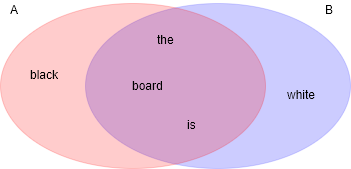
\includegraphics[scale=0.7]{bow_venn}
	\caption{Venn diagram with the BoW representation of $T_1$ and $T_2$.}
	\label{fig:bow_venn}
\end{figure}

So for example, by using the Jaccard similarity:

\begin{equation}
	\jaccsim(A, B)= \frac{3}{5}
\end{equation}

Over a half: they look close. If we used the Hamming distance instead, we would (almost always) get a number very close to 1, because we're using a minuscule part of the universe set (in our case, the English dictionary), thus (almost) all words are absent from the sets.

Now, our objective is to construct a scheme over web-pages that implement the Jaccard similarity.\\
Our pre-processing step: Choose a permutation (or total ordering) $\pi \in \order(A \cup B)$ \uar. To construct said order is a simple task, as we can see with the following algorithm.

Algorithm for sampling a $\uar$ permutation $\pi$ of $[n]$, where $[n]$ is a numeric representation of $U$, and using it to compute the hash of $A$:
\begin{lstlisting}[caption={min hash or shingles algorithm},label={lst:min_hash}]
	MinHash($A$):
	// preprocessing
	$S$ := $[n]$
	$\pi$ := empty sequence
	while $S \neq \emptyset$:
		pick $i \in S \ \uar$
		append $i$ to $\pi$
		remove $i$ from $S$
	end
	// computing hash
	$h_\pi(A)$ := minimum element of A, accordig to $\pi$
	return $h_\pi(A)$
\end{lstlisting}

\begin{proof}[Proof of uniform choice of $\pi$]
	\begin{align*}
	\Pr{X = \pi} &= \frac{1}{s}\cdot\frac{1}{s-1}\cdot\dots\cdot 1\\
	&= \frac{1}{s!} \Rightarrow X \in \unifdist(\permut(A \cup B))
	\end{align*}
\end{proof}

So, from $\pi$, we obtained the following definition:
\begin{defn}[Hashing function]
	\begin{equation}
	h_\pi \in \mathcal{P}(U) \to U : h_\pi(A) = min_\pi(A)
	\end{equation}
\end{defn}

In other words, we take the ``minimum'' in A according to the ordering specified by $\pi$.

\begin{obs}
	A simple but useful observation would be:
	\begin{equation}
	\forall A \subseteq U \Rightarrow h_\pi(A) \in A
	\end{equation}
\end{obs}

\begin{ex}
	\begin{equation*}
		\pi = (black, the, is, white, board) \wedge A = \{the, black, board, is\} \Rightarrow h_\pi(A) = black
	\end{equation*}
\end{ex}

Thus, we say that $A$ is similar to $B$ iff $h_\pi(A)=h_\pi(B)$.
Recall that $A$ and $B$ are fixed, $\pi$ is the focus of this definition. What can be said about $\Pr{h_\pi(A)=h_\pi(B)}$? Looking at a corresponding Venn diagram [\ref{fig:bow_venn}]:
\begin{itemize}
\item $A \cap B = \emptyset \Rightarrow \Pr{h_p(A)=h_p(B)} = 0$; they have no words in common, so their hashes must be different, independently of the chosen order;
\item $A = B \Rightarrow \Pr{h_p(A)=h_p(B)} = 1$; this time, all words are in common, so their hashes must coincide, again, independently of the chosen order;
\item Otherwise, since $\pi$ is chosen \uar, the probability that the hashes are equal has the same meaning of the probability of finding the lowest element of A and B in the intersection with respect of the union (and not in $U$ as a whole, as our previous observation suggests), which is the Jaccard similarity of $A$ and $B$ by its very definition:
\begin{align*}
	\Pr{h_\pi(A)=h_\pi(B)} &= \frac{\Pr{\min(A) \in A \cap B \wedge \min(B) \in A \cap B}}{\Pr{\min(A) \in A \cup B \wedge \min(B) \in A \cup B}}\\
	&= \frac{\abs{A \cap B}}{\abs{A \cup B}} = \jaccsim(A, B).
\end{align*}
\end{itemize}

\textit{Possible question about third point}: Why not respect to the universal set? because $A$ and $B$ will have hashes which, as we observed earlier, do not live outside the union: the union between $A$ and $B$ is our true set of outcomes when hashing either $A$ or $B$.

Now, if $h_\pi$ is evaluated only once over a given permutation, only a binary response can be obtained. In order to obtain the probability value without resorting to compute unions and intersections, we can repeat evaluation over different permutations; this can be regulated by the \textbf{Chernoff-Hoeffding bound}:

Let $A, B \subseteq U$, and $X_{1 \dots n} \in \coin(p)$ \iid, with $\Pr{X_i=1}=p$ and $\Pr{X_i=0}=1-p$, with each $X_i$ defined over a distinct element of $\Pi \subseteq \mathcal{P}erm(U)$, such that $X_i \mapsto 1 \Leftrightarrow A \sim_{\pi_i} B, 0\ otherwise$, then:
\begin{equation} \label{chernoff_hoeffding}
\Pr{\abs{avg_{i=1}^{n}(X_i - p)}\geq\varepsilon} \leq 2e^{-n\varepsilon^2}
\end{equation}
In other words, the difference between the average of the $X_i$ (i.e., the average of the empirically observed results) and their exact probability is greater then $\varepsilon$ only with a very small probability.

So, how many trials (evaluations, observations) are needed to have a good estimate of the similarity? That is, what is a good value for $n$?\\
Let $
	X_i=\begin{cases}
	1 & \text{if}\ h_{\pi_i}(A)=h_{\pi_i}(B)\\
	0 & \text{otherwise}\\
	\end{cases} $
and $\Pr{X_i=1} = \jaccsim(A,B)=p$; we can apply the Chernoff bound on $X_i$ to compute our $n$.\\
If our database has $m$ pages (sets) to store, we can chose $\displaystyle n = \frac{\lg{\frac{2m}{\delta}}}{\varepsilon^2}$ to get a high probability of making zero errors; $\delta$ and $\varepsilon$ are parameters we can set to adjust the size of $n$: even if the bound gives us a high probability for a quite small $n$, we can choose an even smaller $n$ if we can accept big errors for very few pages.

We can now observe that the min hash algorithm [\ref{lst:min_hash}] is efficient: instead of comparing two entire pages, it only compares $n$ integers.

\section{A case study: Comparing DNAs}

In the previous case study, we considered small subsets of the universe set: each web page has only few words with respect to the whole English language.\\
However, there are cases in which the overlays between two subsets are often relevant, for example, if we want to compare the DNA of two people.\\
In such cases, the Hamming similarity is preferable (more significant) to the Jaccard similarity.

We can describe two DNA sequences $A$ and $B$ as two arrays of size $n$, in which each position corresponds to a certain component of the DNA, and contains a 1 if that component is present in that sequence and a 0 if it's absent.
\begin{align*}
	\hammsim(A,B) &=
	\frac{\abs{A \cap B} + \overline{\abs{A \cup B}}}{n}\\
	&= \frac{\text{number of common } 1s + \text{number of common } 0s}{n}
\end{align*}

To get our hash function we pick an index $i\in[n]$ \uar, and we define\\
$ h_i(A)=\begin{cases}
	1 & \text{if}\ i \in A\\
	0 & \text{otherwise}\\
\end{cases} $. \label{hamming_hash}

\begin{ex}
	We have two DNA sequences $A$ and $B$ such that $A:=$
	\begin{tabular}{|c|c|c|c|c|c|c|c|}
		\hline
		0 & 0 & 0 & 1 & 1 & 0 & 0 & 1 \\
		\hline
	\end{tabular},
	$B:=$
	\begin{tabular}{|c|c|c|c|c|c|c|c|}
		\hline
		0 & 1 & 1 & 0 & 0 & 1 & 1 & 1 \\
		\hline
	\end{tabular} and $n:=8$, so we can write $A$ and $B$ as $A=\{4,5,8\},\\ B=\{2,3,6,7,8\}$ using the positions with a $1$ inside (starting from $1$).\\
	If we randomly choose $i=8$, we obtain $h_i(A)=h_i(B)=1$, so we can conclude that $A$ and $B$ are similar.
\end{ex}


Now we can see that the probability that two hashes are equal is the Hamming similarity:
\begin{align*}
	\Pr{h_i(A)=h_i(B)} &= \frac{\Pr{A[i]=B[i]}}{n} \\
	&= \frac{\Pr{(A[i] \text{ and } B[i] \text{ are both } 1) \vee (A[i] \text{ and } B[i] \text{ are both } 0 )}}{n} \\
	&= \frac{\abs{A \cap B} + \overline{\abs{A \cup B}}}{n} = \hammsim(A,B)
\end{align*}

It's possible to obtain a good estimate of the similarity by repeating the test an appropriate number of time, given by the Chernoff Bound.

\section{LSH formalization}

First let us focus around the hash function as an object: its true purpose in a scheme is to classify objects based on how much they ``look like'', whatever this means in the chosen similarity's terms. Therefore, in our theoretical analysis, the codomain of a hash function is not that important; what is important is how the function partitions its own domain, $U$. In a sense, we're interested only in the partitions of $U$ themselves, not in the functions that generate them.

Why have we dealt with functions back then? Moving from a purely mathematical perspective to a more computational one, what is usually done for measuring similarities is sampling some object's characteristics, and observe how ``distant'', or else ``similar'' they are. This is done by means of some program; and programs are (oh so) easily associated with functions. The computational approach gives a more intuitive vision of the problem we're confronting ourselves with.

Still, what could happen, is to have a couple of functions that map values into wildly different codomains, but partition $U$ in exactly the same way! And in our journey, we're just interested in classifying objects; so these kind of ``duplicate'' functions are, well, useless (unless we delve in complexity studies, but that's out of our scope).

So, let us reform the foundations by taking as our core object a universe partition, instead of a universe-domained hash function. First, though, we need to formalize what a similarity is, and to get to a good definition, we have to carefully select them from their space $U^2 \to [0, 1]$. It should be noted that the codomain might very well be $\real$ itself, but to get some bearings we'll treat an image of 1 as a complete equivalence between two objects, and 0 for complete difference, with the interval expressing the degree of similarity.

Let $U$ be a set, and $S \in U^2 \to [0, 1]$ a symmetric function; then $S$ is called a \textbf{similarity} over $U$.
% TODO Still incomplete, need the trineq on 1-S

Tidbit: Let $f \in A^n \to B$, then f is \textbf{symmetric} iff \textit{argument order does not change the image}. % COMMUTATIVITY? Kinda...

\ex \begin{align*}
	& U=2^{[n]}=\left\lbrace A | A \subseteq [n] \right\rbrace \\
	& S=\jaccsim \\
	& S\left( \left\lbrace 1,2 \right\rbrace , \left\lbrace 2,3 \right\rbrace \right) =\frac{1}{3}
\end{align*}

% A scheme-similarity defines a partition over U
A \textbf{LSH scheme} over $U$ is a probability distribution over the partitions of $U$.

\ex We can apply the min-hash scheme [\ref{lst:min_hash}] to the Jaccard Similarity. With $U=[3]$ and $\pi = 1<2<3$, the function maps each subset of $U$ to a hash as follows:
\begin{align*}
	\emptyset &\mapsto \perp \text{(the hash of the empy set is a special symbol)} \\
	\{1\}, \{2,1\}, \{1,3\}, \{1,2,3\} &\mapsto 1 \text{ (all sets containing 1 have hash 1)} \\
	\{2\}, \{2,3\} &\mapsto 2 \text{ (all remaining sets containing 2 have hash 2)} \\
	\{3\} &\mapsto 3 \text{ (all remaining sets containing 3 have hash 3)}
\end{align*}
thus defining 4 partitions over $U$.

\ex Similarly, we can apply the function based on the Hamming Similarity we saw in [\ref{hamming_hash}] to the same set $U=[3]$ and see we get new partitions. We choose $i = 2$ \uar, the function maps each subset of $U$ to a hash as follows:
\begin{align*}
\{2\}, \{2.1\}, \{2,3\}, \{1,2,3\} &\mapsto 1 \text{ (all sets containing $i$ have hash 1)} \\
\emptyset, \{1\}, \{3\}, \{1,3\} &\mapsto 0 \text{ (all remaining sets have hash 0)}
\end{align*}
thus defining 2 partitions over $U$.

Let's make some other considerations about what we have just seen.

%%%%%%%%%%%%%%%%%%%%

% Intuitive: a hash function's purpose is to map arguments that are very similar to the same value

% Hash function: $h \in U \to (*)$ such that the domain's representation is 'sensibly smaller' than U (h is NOT injective by this intuition - not true, injective functions are used as hash functions in pathological cases...)

% Insight: A hash function seems to complicate definitions more than a simple equivalence relation, but it models programs/algorithms more effectively, which is our focus here

\obs Given a similarity $\phi$, a LSH scheme is a family of hash functions $H$, coupled with a probability distribution $D$ over $H$ such that, chosen a function $h$ from the family $H$ according to $D$, $h$ satisfies the property $\Pr{h(a)=h(b)} = \phi(a,b) \forall a,b \in U$. \\
In other words, let $S \in U^2 \to [0, 1]$ be a similarity, and H be a RV over a family of hash functions over U, then H is a LSH scheme iff $\Pr{H(a)=H(b)} = S(a,b) \forall a,b in U$

% Brainlamp: I can extend the domain of H to the whole hashfunction class by setting the outsiders' probability to 0...
%%%%%%%%%%%%%%%%%%%%%%%%%%%%%%%%%%%%


% Note: some partitions will never be a result of a hash function % Hah, not so sure...

% Other note: some form of transitivity must hold. (So yeah, we're dealing with an equivalence relation in the guise of a function with arbitrary codomain)

%\

% INSIGHT
\obs Preprocess and hash function (aka a scheme) determine the similarity function (most people attempt to do the reverse)

% MAJOR INSIGHT:
\obs In the previous webpage example [\ref{sec:web-page-indexing}], we're not dealing with a single hashing function, but with a family of functions each built with its own word permutation: the scheme distributes over the permutations of the union!
% Now, do all permutations induce unique partitions?

%\

% Wrapup:
Before going on, let's recap what we have discussed so far: \\
A LSH scheme for a similarity $S$ is a prob. dist. over $U$'s partitions such that 
\begin{equation}
	\forall A, B \in  U \Rightarrow \Pr{A\sim_p B}_p = S(A, B) = \Pr{h(A)=h(B)}_h
\end{equation}
where $p$ is a partitioning of $U$ and $\sim_p$ means $A$ and $B$ are in the same partition.

Another possible definition: Given $s \in U^2 \to [0,1]$ a similarity, then we define $X$ to be a LSH scheme for $s$ as the following:
\begin{equation}
X \in \probdist(\powerset(U)) : \forall A, B \in U \implies \expect(A\sim_X B) = S(A, B)
\end{equation}

\textit{Challenge}: Can we find a LSH scheme for an arbitrary S function? NO

\ex \label{ex:transitivity} Given a universe set $U = \{a, b, c\}$ and a similarity function $S$ s. t.	$S \in U^2 \rightarrow [0, 1] : S(a, b) \mapsto 1, S(b, c) \mapsto 1, S(a, c) \mapsto 0$ we don't have an LSH, since we're violating transitivity:
Translating into probabilities and using equality's transitivity, we obtain: $\Pr{h(a), h(c)}=1$, which contradicts the third mapping.

\section{More distances}
Let $A \vartriangle B = (A-B) \cup (B-A)$.

\begin{defn}[Dice similarity]
	\begin{equation}
	\displaystyle D(A, B) = \frac{|A\cap B|}{|A\cap B| + \frac{1}{2}|A\vartriangle B|}
	\end{equation}
\end{defn}

\begin{defn}[Anderberg similarity]
	\begin{equation}
	\displaystyle An(A, B) = \frac{|A\cap B|}{|A\cap B| + 2|A\vartriangle B|}
	\end{equation}
\end{defn}

\begin{defn}[Generalizing Jaccard, Dice and Anderberg]
	\begin{equation}
	\displaystyle S_\gamma(A, B) = \frac{|A\cap B|}{|A\cap B| + \gamma|A\vartriangle B|}
	\end{equation}
\end{defn}

By this third definition we can obtain $\jaccsim$ with $\gamma = 1$, $D$ with $\gamma=\frac{1}{2}$, and $An$ with $\gamma = 2$. It would be useful to know for which values of $\gamma$ there exists an LSH for $S$; the next lemma helps us finding an answer:

\begin{lem}[Charikar]
	If a similarity $S$ admits an LSH, then the function $d := 1 - S$ must satisfy the triangular inequality, i.e. it is a metric\footnote{In most cases, similarities are actually defined as inverses of some existing metric.}:
	\[
		\forall A, B, C \in U \quad d(A, B) \leq d(A, C) + d(B, C)
	\]
\end{lem}

\begin{proof}
	Let $E_{XY}$ be the event ``$h(X) \neq h(Y)$"; since $S$ admits a LSH, we have:
	\begin{align*}
		d(A,B) &= 1-S(A,B) = \Prs_h{E_{AB}} = p_1 + p_2 + p_3 + p_4 \\
		d(A,C) &= 1-S(A,C) = \Prs_h{E_{AC}} = p_1 + p_3 + p_5 + p_7 \\
		d(B,C) &= 1-S(B,C) = \Prs_h{E_{BC}} = p_1 + p_2 + p_5 + p_6
	\end{align*}
	with the probabilities $p_i$ defined as in the following table, where an $X$ under the ``may exist" column means that the corresponding probability is $0$ (it happens because transitivity generates contradictions, see example [\ref{ex:transitivity}]):

	\vspace{1ex}
	\begin{tabular}{lllll}
		& $E_{AB}$ & $E_{AC}$ & $E_{BC}$ & may exist             \\
		$p_1$ & T         & T         & T         & $\checkmark$ \\
		$p_2$ & T         & T         & F         & $\checkmark$ \\
		$p_3$ & T         & F         & T         & $\checkmark$ \\
		$p_4$ & T         & F         & F         & X            \\
		$p_5$ & F         & T         & T         & $\checkmark$ \\
		$p_6$ & F         & T         & F         & X            \\
		$p_7$ & F         & F         & T         & X            \\
		$p_8$ & F         & F         & F         & $\checkmark$
	\end{tabular}

	Hence we have
	\begin{equation*}
		d(A,C) + d(B,C) = 2p_1 + p_2 + p_3 + 2p_5 \geq p_1 + p_2 + p_3 = d(A,B)
	\end{equation*}
	and so $1-S$ doesn't comply with the triangular inequality.
\end{proof}

\begin{cor}
	Dice's similarity cannot admit a LSH scheme.
\end{cor}

\begin{proof}[Proof by counterexample]
	Assume $A = \{1\}, B = \{2\}, C = \{1, 2\}$, then use the triangular inequality over the distances:
	\begin{align*}
		& D(A, C) = \frac{2}{3},\ D(B, C) = \frac{2}{3},\ D(A, B) = 0 \\
		& d(A, B) = 1 - D(A, B) = 1 > \frac{2}{3} = (1 - D(A, C)) + (1 - D(B, C)) = d(A, C) + d(B, C)
	\end{align*}
	hence it doesn't comply with the triangular inequality. By Charikar's lemma, $D$ cannot admit a LSH scheme.
\end{proof}

This proof also sheds some insight on $\gamma$-similarities: parameterizing this counterexample with $S_\gamma$, a bound on $\gamma$ for LSHable functions can be obtained. Let $A = \{1\},\ B = \{2\},\ C = \{1, 2\}$ and $S_\gamma(A, C) = \frac{1}{1 + \gamma},\ S_\gamma(B, C) = \frac{1}{1 + \gamma},\ S_\gamma(A, B) = 0$. Then:
\begin{align*}
	1 =&\ 1 - S_\gamma(A, B) 							& \tag{$S_\gamma(A, B) = 0$}\\
	  >&\ (1 - S_\gamma(A, C)) + (1 - S_\gamma(B, C)) 	& \tag{trineq on $1 - S_\gamma$, which is a metric by Charikar's lemma}\\
	  =&\ 2 \left( 1 - \frac{1}{1 + \gamma} \right)		& \\
	  =&\ \frac{2\gamma}{1 + \gamma} 					&
\end{align*}
which entails:
\[
	1 > \frac{2\gamma}{1 + \gamma} \quad \implies \quad \gamma < 1
\]
Hence, if $\gamma < 1$, the triangular inequality doesn't hold, so no LSH can exist, as in the case of the Dice similarity.

	
\section{Probability generating functions}
	
A probability generating function (\pgf) is a power series representation of a given discrete probability distribution:

\begin{defn}
	Given a discrete RV $X$, its \pgf{} is the function:
	\[
		\mathcal{G}en_X(\alpha) = \sum_{x = 0}^{\infty} \Pr{X = x} \alpha^x
	\]
	(note that all outcomes appear by their probability).
\end{defn}

To get back to the corresponding probability mass function : $\displaystyle \Pr{X = \omega} = \frac{\mathcal{D}_x^\omega(\mathcal{G}en_X(0))}{x!}$, where $\mathcal{D}$ denotes the overline-x-th derivative on x of the generating function. From another perspective, a \pgf{} $f$ is a function such that:
\[
	f(x) = \sum_{i = 0}^{\infty} p_i x^i
\]
where $p_i \geq 0\; \forall i$ and $\sum_{i = 0}^{\infty} p_i = 1$. In turn the corresponing mass function is:
\[
	\Pr{X = \omega} = \frac{\mathcal{D}_x^\omega(\sum_{i = 0}^{\infty} p_i x^i)}{x!}
\]


\section{Constructing schemes from \pgf s}

%% So it actually matches the previous wikipedian def
\textit{Recap}: Given a universe $U$, a function $S \in U^2 \to [0, 1]$ is said to be a \textbf{LSHable similarity} iff exists a prob. distr. over (a family/subset of) the hash functions in $U$, such that: 
\begin{equation}
\forall \{X, Y\} \in \binom{U}{2}\ \ \Prs_h{h(X)=h(Y)} = S(X, Y)
\end{equation}

\begin{thm} \label{t:pgf_1}
	If a similarity $S$ is LSH-able and $f$ is a \pgf, then $f(S)$ is LSHable:
	\[
		f(S) := T \in U^2 \to [0, 1] : \forall \{A, B\} \in \binom{U}{2}\ \ T(A, B) = f(S(A, B))
	\]
	\[
		f(S(A, B)) = (f(S)) (A, B) =: T (A,B)
	\]
\end{thm}

% TODO check
% Afterthought: Are we ``applying" a probability distribution over a similarity (which in turn, since it is lshable, means it has a probdist over a subset of hashfunctions)?

% TODO check
%Afterthought: could we just prove that probability distributions are composable? lshability could be just a carried-over property...
%%%%%%%%%%%%%%%%%%%%%%%%%%%%%%%%%%%%%%%%%%%%%%%%%%%%%%%%%%%%%%

The proof is inductive and makes use of four lemmas presented here. The first one forms the basis of induction:
\begin{lem}[L1]\label{l:pgf_1}
	The similarity $O \in U^2 \to [0, 1] : O(A, B) \mapsto 1$ admits a LSH.
\end{lem}

\begin{proof}
	The scheme consists of always choosing the constant hash function $h_1$:
	\[
		h_1 \in U \to [0, 1] : A \mapsto 1 \qedhere
	\]
\end{proof}


\begin{lem}[L2]\label{l:pgf_2}
	If $S$ and $T$ are similarities over $U$ that have a scheme, then $S \cdot T : (S \cdot T)(A, B) = S(A, B) \cdot T(A, B)$ has a scheme; in other words, LSHability is preserved on ``concatenation''.
\end{lem}

\begin{proof}
	The proof is constructive, here is the algorithm:
	\begin{itemize}
		\item[] Hash function for $S \cdot T$:
		\item Sample $h_S$ from the LSH for $S$
		\item Sample $h_T$ independently from the LSH for $T$
		\item Return the hash function $h$ such that $A \mapsto (h_S(A), h_T(A))$
	\end{itemize}

	For any $A$ and $B$ picked from $U$:
	\begin{align*}
		&\  \Prs_h{h(A) = h(B)} 										  & \\
		=&\ \Prs_{h_S}{h_S(A) = h_S(B)} \cdot \Prs_{h_T}{h_T(A) = h_T(B)} & \tag{by independency of $S$ and $T$} \\
		=&\ S(A, B) \cdot T(A, B)										  &
	\end{align*}
	which means that $h$ is effectively a LSH scheme for $S \cdot T$.
\end{proof}

\begin{lem}[L3]\label{l:pgf_3}
	If $S$ is LSHable, then $S^i$ is LSHable $\forall i \in \mathbb{N}$.
\end{lem}

\begin{proof}
	Proven by induction over $i$:
	\begin{itemize}
		\item Base ($i = 0$): $S^0 = O$ has a scheme by lemma \ref{l:pgf_1};
		\item Induction ($S^i$ is LSHable $\implies S^{i+1}$ is LSHable: True because $S^{i + 1} = S \cdot S^i$, and both operands have a scheme by lemma \ref{l:pgf_2} and by inductive hypothesis.
	\end{itemize}
\end{proof}

\begin{lem}[L4]\label{l:pgf_4}
	If $p_0, p_1, \dots, p_i, \dots$ is such that $\sum_{i = 0}^{\infty} p_i = 1$, $p_i \geq 0 \ \forall i$, and $S_0, S_1, \dots, S_i, \dots$ are lshable similarities, then $\sum_{i = 0}^{\infty} p_i S_i$ is lshable.
\end{lem}

\begin{proof}

	\todo{

	Proven by construction:
	\begin{enumerate}
		\item First, sample $i*$ at random from $\mathbb{N}$ with probability $p_0, ..., p_i, ...$;
		\item Then, sample $h$ from the hash functions (LSH) of $S_{i*}$ (that is, we are choosing which LSH to use);
	\end{enumerate}
	Therefore:
	\begin{align*}
		&\  \Prs_h{h(A) = h(B)} \\
		=&\ \sum_{i = 0}^{\infty} p_i \cdot S_i(A, B) \\
		=&\ \sum_{i = 0}^{\infty}(\Pr{i = i*} \cdot \Prs_h{h(A) = h(B) \mathrel{|} i = i*}) \qedhere
	\end{align*}
	}
\end{proof}

This lemma is useful if we need a weighted average:
\[
	W(A,B) = \sum_{i=0}^{\infty}(p_i S_i(A, B))
\]

\begin{proof}[Proof of the theorem \ref{t:pgf_1}]
	We want to prove that $\sum_{i = 0}^{\infty} p_i S^i$ has a scheme. By L3 [\ref{l:pgf_3}] we know $S^i$ has a scheme, and by L4 [\ref{l:pgf_4}] we know the sum is lshable.
\end{proof}	


\subsubsection{Use cases}

\obs This theorem tells us how to build a LSH: by concatenating the results of different hash functions, keeping the output small. I.e. PGF is an approach for making schemes for similarities from other schemes.
\[
	\sum_{i=1}^{a}(2^{-i} \cdot x^i)
\]

Another consequence of the theorem is revealed when the statement is applied to the Jaccard similarity.

Our function is $f_\gamma$, with $\gamma > 1$, defined as
\begin{equation} \label{eq:pgf_jacc}
	\displaystyle f_\gamma(x) = \frac{x}{x+\gamma(1-x)}
\end{equation} \\
In order to proof $f_\gamma$ is a PGF, we have to demonstrate that the coefficients represent a probability distribution: i.e., they are all positive and they sum to zero. \\
By applying the Taylor series expansion to [\ref{eq:pgf_jacc}], we get \\
$\displaystyle
	f_\gamma(x) = \sum_{x=1}^{\infty}\left(\frac{\left(1-\frac{1}{\gamma}\right)^i}{\gamma -1}x^i\right)
$; now $f_\gamma$ is a power series, so all the coefficients are positive. \\
In order for the sum of the coefficients to be equal to 1, the numerator must be equal to the denominator: \\
$\displaystyle \sum_{i=1}^{\infty} \left(\frac{\left(1-\frac{1}{\gamma}\right)^i}{\gamma -1} \right) = 1 \Rightarrow \sum_{i=1}^{\infty} \left( \left(1-\frac{1}{\gamma}\right)^i \right) = \gamma -1$. \\
Indeed we have:
\begin{flalign*}
	\sum_{i=1}^{\infty}\left(1 - \frac{1}{\gamma}\right)^i
	&= \left(1 - \frac{1}{\gamma}\right)\sum_{i=0}^{\infty}\left(1 - \frac{1}{\gamma}\right)^i &&\\
	&=^{\left(*\right)} \left(1 - \frac{1}{\gamma}\right) \frac{1}{1 - \left(1 - \frac{1}{\gamma}\right)} &&\\
	&= \frac{\gamma -1 }{\gamma}\frac{1}{1/\gamma} = \gamma -1 &&
\end{flalign*}
where the step marked with $\left(*\right)$ is due to the equality $\sum_{i=0}^{\infty} \alpha^i = \frac{1}{1-\alpha}$. \\
And with this we proved that $f_\gamma$ is a PGF.

Now we can apply PGF to a similarity $S_\gamma$:
\begin{align*}
f_\gamma (S_\gamma(A, B))
&= f_\gamma \left( \frac{\abs{A \cap B}}{\abs{A \cup B}} \right) \\
&= \frac{\frac{\abs{A \cap B}}{\abs{A \cup B}}}
	{\frac{\abs{A \cap B}}{\abs{A \cup B}} +
		\gamma \frac{\abs{A \cup B} -
			\abs{A \cap B}}{\abs{A \cup B}}} \\
&= \frac{\abs{A \cap B}}
	{\abs{A \cap B} + \gamma \abs{A \vartriangle B}}
	= S_\gamma(A, B)
\end{align*}
which in turn is LSH-able


\section{A mention of the sketches}

Like LSH, they're a means for simplify the storage of data; they are slower than LSH but allow you to keep interesting information in a small space.

\defn[Sketch] A sketch is a representation of big objects with small images. They can be used to retrieve interesting information about original objects without regain the whole original objects (i.e. they are not compression algorithms).

\ex It's possible to go back to $\abs{A \cap B}$ from only $|A|, |B|, h(A), h(B),$ $\jaccsim(A,B)\pm\varepsilon$. Note that $\jaccsim(A,B)\pm\varepsilon$ can be obtained from $h(A), h(B)$ by applying the Chernoff Bound, and the other data need only few bits to be stored.

\ex It's possible to approximate $\frac{\abs{A \cap B}}{\abs{A \cap B} + \frac{1}{2}\abs{A \vartriangle B}}$ with
	$\frac{1}{2} \cdot \abs{A \cup B} + \frac{1}{2} \cdot \abs{A \cap B}$.

% TODO check
% --------------------------------------------------------------
% ??sorensen dice??cosine similarity?? inner product??johnson-lindenstrauss??
	
%a sketch is n instance of a pgf which can be used to implement other similarities NONONONONOO
	
	
	
\section{Approximation of non-LSHable functions}

What can we do if there is no LSH for the similarity we want/need to use? We can approximate a function without a LSH with an LSHable one. For example, we can approximate $S_\gamma$ with $\jaccsim$ with an error of $\frac{1}{\gamma}$.

% TODO check
\begin{thm}
	Let $f$ be a \pgf, and $\alpha \sim \coin(p)$. Define the following function:

	\[
		f_\alpha(S) = \begin{cases}
			\alpha \cdot f(S)		& \text{with probability $p$} \\
			(1 - \alpha) \cdot T	& \text{with probability $(1 - p)$}
		\end{cases}
	\]

	where $S$ is a similarity grouping every element under a single class, and T is another smiliarity where each element has its own distinct class.
\end{thm}

When $\alpha = 1$, $f_\alpha$ induces a banal partition over its domain, whereas with $\alpha = 0$ the induced partition is punctual. The hash functions that can implement such a function would be a constant one for $S$, and an identity function for $T$ (remember that in $T$'s case, $T(x, x) = 1$). However this is not a good scheme, because we're not shrinking data.

% TODO ???
% GOTO %&

\begin{defn}[Distortion]
	Let $S: U^2 \to [0, 1]$ be a similarity, then its \textbf{distortion} is the minimum\footnote{If $U$ isn't finite, there is no actual minimum; care should be taken in choosing an appopriate bound close to the infimum} $\delta \geq 1$ s.t. $\exists$ an LSHable similarity $S'$ s.t. $\forall {A, B} \in \binom{U}{2}$ $\frac{1}{\delta} \cdot S(A, B) \leq S'(A, B) \leq S(A, B)$.
\end{defn}

Note that $S'$ is the LSHable similarity closest to $S$; the more $\delta$ is near to $1$, the closer $S'$ is to $S$ (i.e. $\delta$ is the \textit{approximation factor}); if $\delta$ tends to $1$, then $S$ is LSHable. For example, where we used $\jaccsim$ to approximate $S_\gamma$, we had $\delta \to \frac{1}{\gamma}$. To check if there is a better approximation, the following lemma is presented:

\begin{lem}[Center lemma] \label{l:center}
	Let $S$ be a LSHable similarity s.t. $\exists \mathcal{X} \subseteq U : \forall \{x, x'\} \in \binom{\mathcal{X}}{2} \ S(x, x')=0$, then $\forall y \in U \ avg_{x \in \mathcal{X}}(S(X, Y)) \leq \frac{1}{\abs{\mathcal{X}}}$.
\end{lem}

\begin{proof}
	Fix $y \in U$. If the hash function $h$ has positive probability in the (chosen) LSH for $S$, then $\forall {x, x'} \in \binom{\mathcal{X}}{2} \ h(x)\neq h(x')$ (otherwise we would have $S(x, x') > 0$). Thus, for all hash functions with positive probability, there can exist at most one $x \in \mathcal{X}$ s.t. $h(x) = h(y)$ (by transitivity of equality). Therefore:
	
	\begin{align*}
		\sum_{x \in \mathcal{X}}S(x, y) &= \sum_{x \in \mathcal{X}}\Prs_h{h(x) = h(y)} \\
		&= \sum_{x \in \mathcal{X}}\sum_{h}\Pr{h \text{ is chosen}} \cdot \overbrace{[h(x) = h(y)]}^{\substack{\text{prob. that $x = y$} \\ \text{with the chosen $h$}}} \\
		&= \sum_h \Pr{h \text{ is chosen}} \cdot \sum_{x \in \mathcal{X}}[h(x)=h(y)] \\
		&\leq \sum_h \Pr{h \text{ is chosen}} = 1 
	\end{align*}

	Thus, $\sum_{x \in \mathcal{X}}S(x, y) \leq 1$, which implies that $avg(S(X, Y)) \leq \frac{1}{\abs{\mathcal{X}}}$.
\end{proof}

$\mathcal{X}$ is a set of the most different objects in $U$ and $y$ is a center in $U$; so the meaning of the lemma is that the average of the distances between each point and the center is $\leq \frac{1}{\abs{\mathcal{X}}}$. Note that $\mathcal{X}$ is actually a (possibly incomplete) section of the partition of $U$ induced by $h$. Also, it trivially follows from the center lemma that:
\[
	\exists \ x^* \in \mathcal{X} : S\left(x^*, Y \leq \frac{1}{\abs{\mathcal{X}}}\right)
\]


\subsubsection{Application to $S_\gamma$}
	
We will now prove what we said about $S_\gamma$'s approximation using the lemma we have just proven. Let us give some definitions:

\begin{itemize}
	\item $S := S_\gamma \text{, with } 0 < \gamma < 1$,
	\item $U := 2^{[n]}=\{S|S\subseteq [n]\}$,  %insieme delle parti?
	\item $\mathcal{X} := \mathcal{P}_1([n])=\{ \{1\}, \{2\}, ..., \{n\} \}$;
\end{itemize}

By definition of $S_\gamma$, we have $S_\gamma(\{i\},\{j\}) = 0 \ \forall i \neq j \in [n]$, since $\{i\} \cap \{j\} = \emptyset$. Let us assume that $T$ (that will be our $S'$) finitely distorts $S_\gamma$, and $T$ is LSHable; then $T(\{i\},\{j\}) = 0 \ \forall \{i, j\} \in \binom{[n]}{2}$, since $S' \leq S_\gamma = 0$. Since $T$ is LSHable we can apply the center lemma:

\begin{align*}
	& \exists \{i\} \in \mathcal{X} \text{ s.t. } T(\underbrace{\{i\}}_\text{our $x^*$}, \underbrace{[n]}_\text{our $y$}) \leq \frac{1}{\abs{\mathcal{X}}} = \frac{1}{n} &&\\
	& S_\gamma(\{i\}, [n]) = \frac{1}{1 + \gamma \cdot (n-1)} = \frac{1}{\gamma \cdot n + (1-\gamma)} &&\\
	& \text{so } \exists i \in [n] \text{ s.t. } S_\gamma(\{i\}, [n]) \geq \frac{1}{\gamma \cdot n + (1-\gamma)} &&\\
	& \text{but } T(\{i\}, [n]) \leq \frac{1}{n} &&\\
	& \text{thus } \frac{1}{\delta} \frac{1}{\gamma \cdot n + (1-\gamma)} = \frac{1}{\delta} S_\gamma(\{i\}, [n]) \leq T(\{i\}, [n]) \leq \frac{1}{n} &&\\
	& \text{hence } \frac{1}{\gamma + \frac{1-\gamma}{n}} = \frac{n}{\gamma \cdot n + (1-\gamma)} \leq \delta &&\\
	& \liminf_{n \to \infty} \delta \geq \frac{1}{\gamma} &&
\end{align*}

i.e. the more $n$ grows, the more $\delta$ approaches $\frac{1}{\gamma}$. Now we know that the distortion bound of $S_\gamma$ is $\frac{1}{\gamma}$.


\subsubsection{Application to the cosine similarity}

Now we would like to apply the same method to the \emph{cosine similarity}, also known as the \emph{inner product similarity}.  Let's start again with some definitions:

\begin{itemize}
	\item $U := \{ \vec{x} \ | \ \vec{x} \in \mathbb{R}_+^n, \ \abs{\abs{\vec{x}}}_2=1 \}$ \ \
	(i.e., $U$ is a positive hypersphere with the center in the origin and the radius equal to 1),
	\item $C \in U^2 \to [0,1]$ s.t. $C(\vec{x}, \vec{y}) = \left\langle \vec{x}, \vec{y} \right\rangle = \sum_{i=1}^n x_iy_i$;
\end{itemize}

Now, we want to know if $C$ has an LSH and, if not, what is its distortion. Define:
\[
	\mathcal{X}=\{ \vec{x}_1, \vec{x}_2, ..., \vec{x}_n \} \text{ , where } x_i(j)=\begin{cases}
		1 & \text{if } i = j \\
		0 & \text{otherwise} \\
	\end{cases} 
\]
or in other terms, $\vec{x}_i=(0,...,0,1,0,...,0)$ with the only 0 in position $i$. Then:

\begin{itemize}
	\item So we have that $\abs{\abs{\vec{x}}}_2=\sqrt{1^2+0^2(n-1)}=1$;
	\item Moreover $C(\vec{x_i}, \vec{x_j})=0 \ \forall i\neq j$;
	\item Let $\vec{y}=\left( \underbrace{\frac{1}{\sqrt{n}}, \frac{1}{\sqrt{n}}, ..., \frac{1}{\sqrt{n}}}_\text{n times} \right)$, then $\abs{\abs{\vec{y}}}_2 = \sqrt{\sum_{i=1}^n y_i^2} = \sqrt{\sum_{i=1}^n \frac{1}{n}}=1$;
	\item So, $C(\vec{x_i}, \vec{y})= \sum_{j=1}^n \left( x_i(j) \cdot y_i(j) \right) = x_i(i) \cdot y_i(i) = \frac{1}{\sqrt{n}}$;
	\item Then $\delta \geq \sqrt{n}$, so, unlike before, the distortion is big and grows bigger with $n$.
\end{itemize}

Some other related examples follow:

\ex \textbf{Weighed Jaccard} is a generalization of $\jaccsim$ for vectors: \\ $\mathcal{WJ}=\frac
	{\sum_i \min(x_i, y_i)}{\sum_i \max(x_i, y_i)}$.

\ex \textbf{Sim Hash} is an LSH scheme similar to the cosine similarity:
\begin{itemize}
	\item $\mathcal{CS}(\vec{x},\vec{y})=
		\cos(\theta_{\vec{x},\vec{y}}) $;
	\item $\mathcal{SH}(\vec{x},\vec{y})=
		1-\frac{\theta_{\vec{x},\vec{y}}}{\pi} $;
	\item $\mathcal{SH}$ is high if the angle $\theta$ is small;
	\item $\frac{\theta_{\vec{x},\vec{y}}}{\pi}$ is the probability that an hyperplane divides $\vec{x}$ and $\vec{y}$, where the hyperplane is a threshold between similar and dissimilar elements of the universe, so it creates a partition of the universe in two sets.
\end{itemize}
